\documentclass[10pt]{article}
\usepackage{amsmath, amssymb, amsfonts} % برای فرمول‌نویسی
\usepackage{breqn} % برای فرمول‌نویسی
\usepackage{amsthm}% برای اضافه کردن محیط proof
\usepackage{subfigure} % اضافه کردن شکل های زیر شکل ها
\usepackage{setspace} % تعیین فاصله بین خطوط
\usepackage{graphicx} % اضافه کردن عکس
\usepackage{multicol} % حروف چینی چند ستونه
\usepackage[margin=1in]{geometry} % تغییر دادن حاشیه دور

\graphicspath{{./pics/}}

\usepackage{xepersian}

\settextfont{XB Yas} % برای ست کردن فونت متن
\setdigitfont{XB Zar} % برای ست کردن فونت اعداد

\setcounter{secnumdepth}{4} % Set Sections' Depth
\setcounter{tocdepth}{4}% Set Table Of Content's Depth

\title{تمرین کامپیوتری ۱ سیستم‌های مخابراتی}
\author{نام و نام‌ خانوادگی : امیرمهدی جعفری فشارکی
\\ \\
شماره دانشجویی : ۹۸۱۰۹۶۴۵ 	\\ \\
تاریخ : ۲۱ آبان ۱۴۰۰}
\date{}
\doublespacing

\begin{document}
	\maketitle
	\pagebreak
	\tableofcontents
	\newpage
	\section{توضیجات اولیه}
	کد‌های مربوط به سوالات در فولدر 
	\lr{Codes}
	قرار دارد و تمامی تصاویر مربوط به سوالات در فولدر 
	\lr{pics}
	قرار دارد.
	همچنین این گزارش با استفاده از
	 \LaTeX
	 تهیه شده است و فایل 
	 \lr{tex}
	 مربوط به آن در فولدر 
	 \lr{Report}
	 قرار دارد.
	\section{کانال چند مسیره}
	کد‌ مربوط به این سوال در 
	\lr{Q1.m}
	قرار داد.
	\subsection{رسم نمودار 
	\lr{x(t)}}
	با نمونه برداری از سیگنال مورد نظر، شکل آن مانند شکل زیر
	می‌باشد.
	\begin{figure}[h]
		\centering
		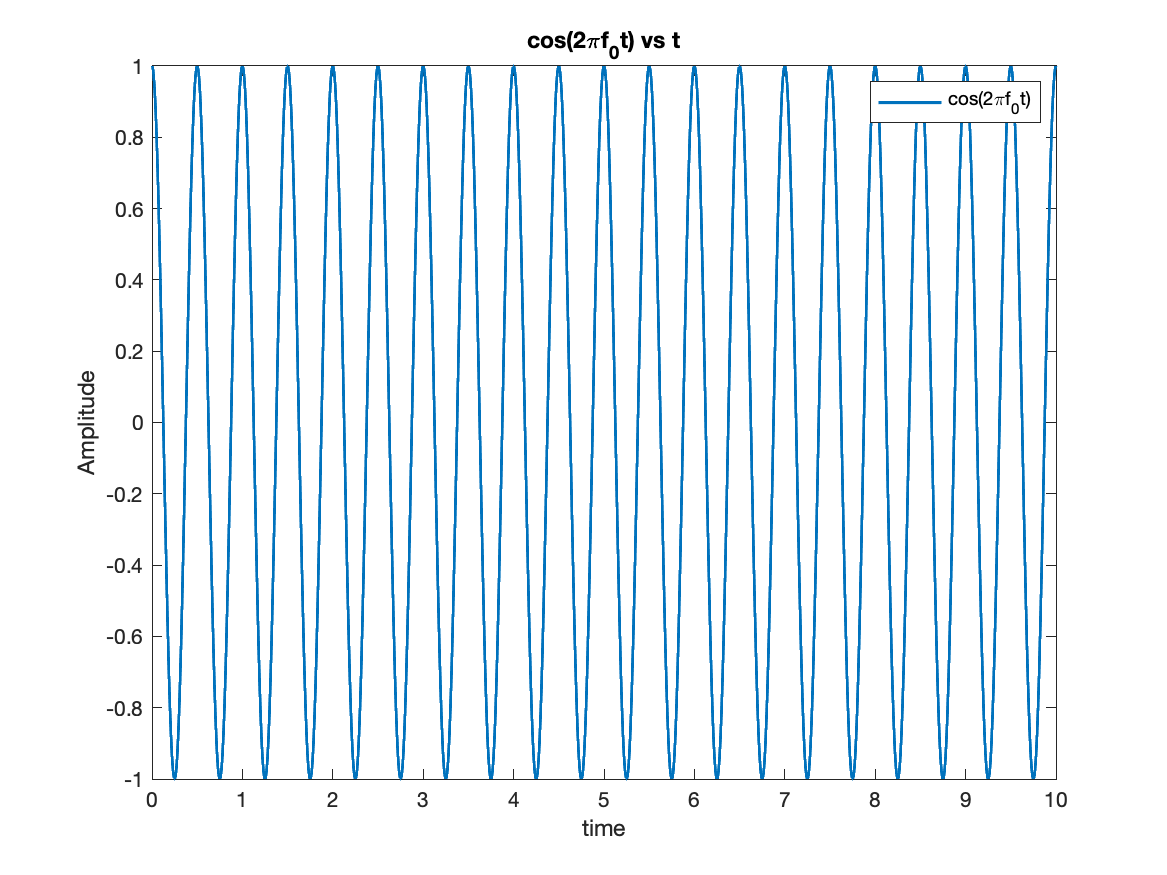
\includegraphics[width=0.9\linewidth]{../pics/q1-1}
		\caption{نمودار سیگنال نمونه برداری شده}
		\label{q1-1}
	\end{figure}
	\newpage
	\subsection{تولید کانال با متغیرهای تصادفی}
	در این بخش همان‌طور که مشاهده می‌شود ابتدا متغیرهای تصادفی مورد نظر تولید با استفاده از توابع rand و normrnd تولید می‌شوند و با رسم شکل به ازای این مقادیر، نمودار اندازه و فاز پاسخ فرکانسی از فرکانس 
	\lr{-5kHz}
	تا
	\lr{5kHz}
	به شکل زیر می‌باشد.
	
	\begin{figure}[h]
		\centering
		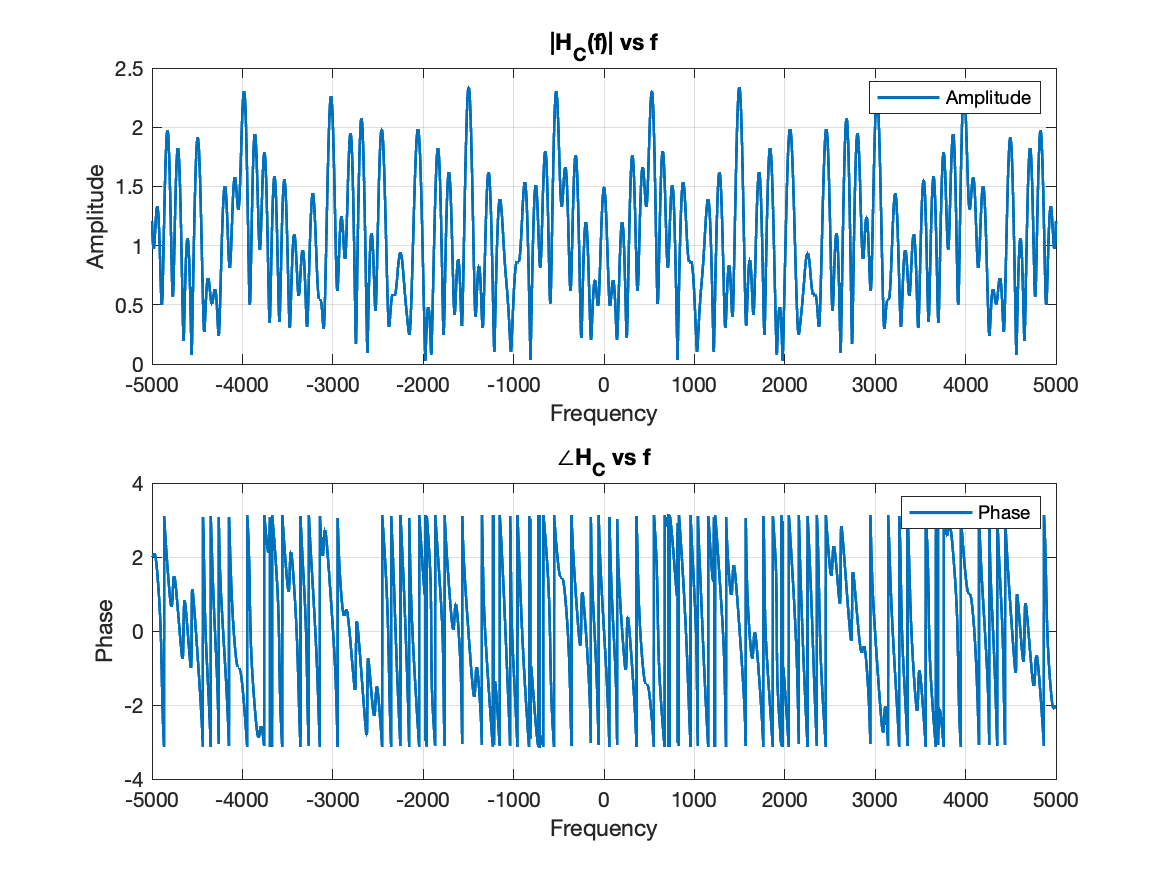
\includegraphics[width=0.9\linewidth]{../pics/q1-2}
		\caption{نمودار اندازه و فاز پاسخ فرکانسی بر حسب فرکانس}
		\label{fig:q1-2}
	\end{figure}
	
	\subsection{رابطه میان فاصله دره‌های پاسخ فرکانسی}
	با رسم اندازه پاسخ فرکانسی به ازای مقادیر مختلف 
	\lr{$T_m$}
	می‌توان مشاهده کرد که فاصله این دره ها با مقدار 
	\lr{$T_m$}
	رابطه عکس دارد. به این دلیل می‌توان حدس زد که رابطه فاصله دره ها با 
	\lr{$T_m$}
	به شکل معادله زیر می‌باشد:
	\[\Delta f \approx \frac{\alpha}{T_m}\]
	
	\noindent
	که در اینجا آلفا خود ضریبی متناسب با پارامتر‌های دیگر مساله می‌باشد.
	همچنین نمودار به ازای چند حالت مختلف به شکل زیر می‌باشد.
	\newpage
	\begin{figure}[h]
		\centering
		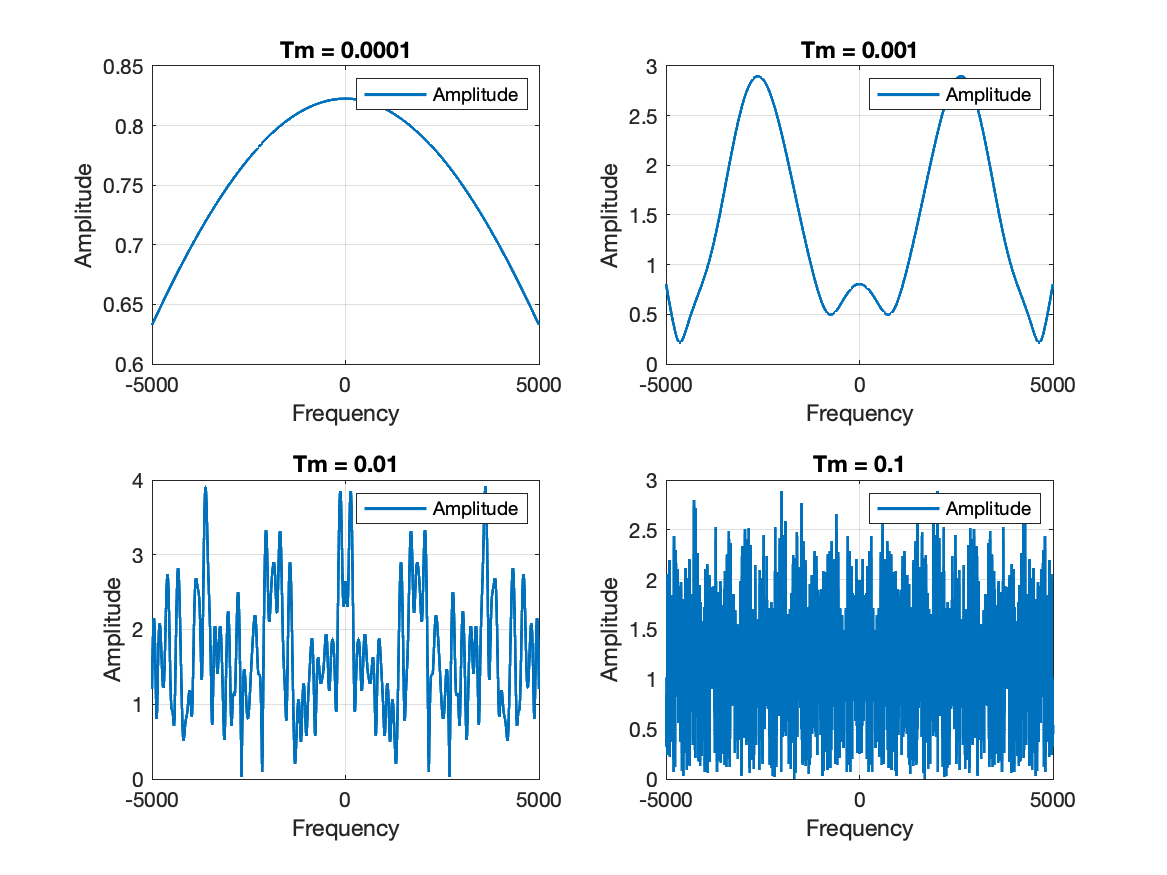
\includegraphics[width=0.9\linewidth]{../pics/q1-3}
		\caption{نمودار اندازه پاسخ فرکانسی برای مقادیر متفاوت 
		\lr{$T_m$}}
		\label{fig:q1-3}
	\end{figure}

\noindent
همان‌طور در شکل
 \ref{fig:q1-3}
 نیز مشخص است با افزایش 
 \lr{$T_m$}
 فاصله ها کاهش پیدا می‌کند و به همین دلیل به ازای 
 \lr{$T_m$}
 خیلی بزرگ فاصله ها بسیار کاهش می‌یابد و به ازای 
 \lr{$T_m$}
 خیلی کوچک، پاسخ فرکانسی کانال تقریبا ثابت شده و تغییرات آن بسیار کم است.
 \newpage
 \subsection{کانال نمونه‌برداری شده}
 در این بخش ابتدا یک تابع به نام 
 \lr{channel\_response}
 تعریف شده است که 
 \lr{N}
 ذکر شده در صورت سوال را به عنوان ورودی گرفته و با استفاده از آن N، پس از هر N نمونه، مقادیر تصادفی کانال را تغییر داده و در نهایت به ازای N مشخص شده، خروجی کانال و زمان را به عنوان خروجی تابع می‌دهد. سپس برای 
 \lr{N}
 های خواسته شده در سوال، این مقادیر رسم شده است. همچنین برای محاسبه پاسخ در هر ثانیه از رابطه 
 \[y(t) = \sum_{i=1}^{n} a_i x(t-\tau_i)\]
 استفاده شده است.
 \begin{figure}[h]
 	\centering
 	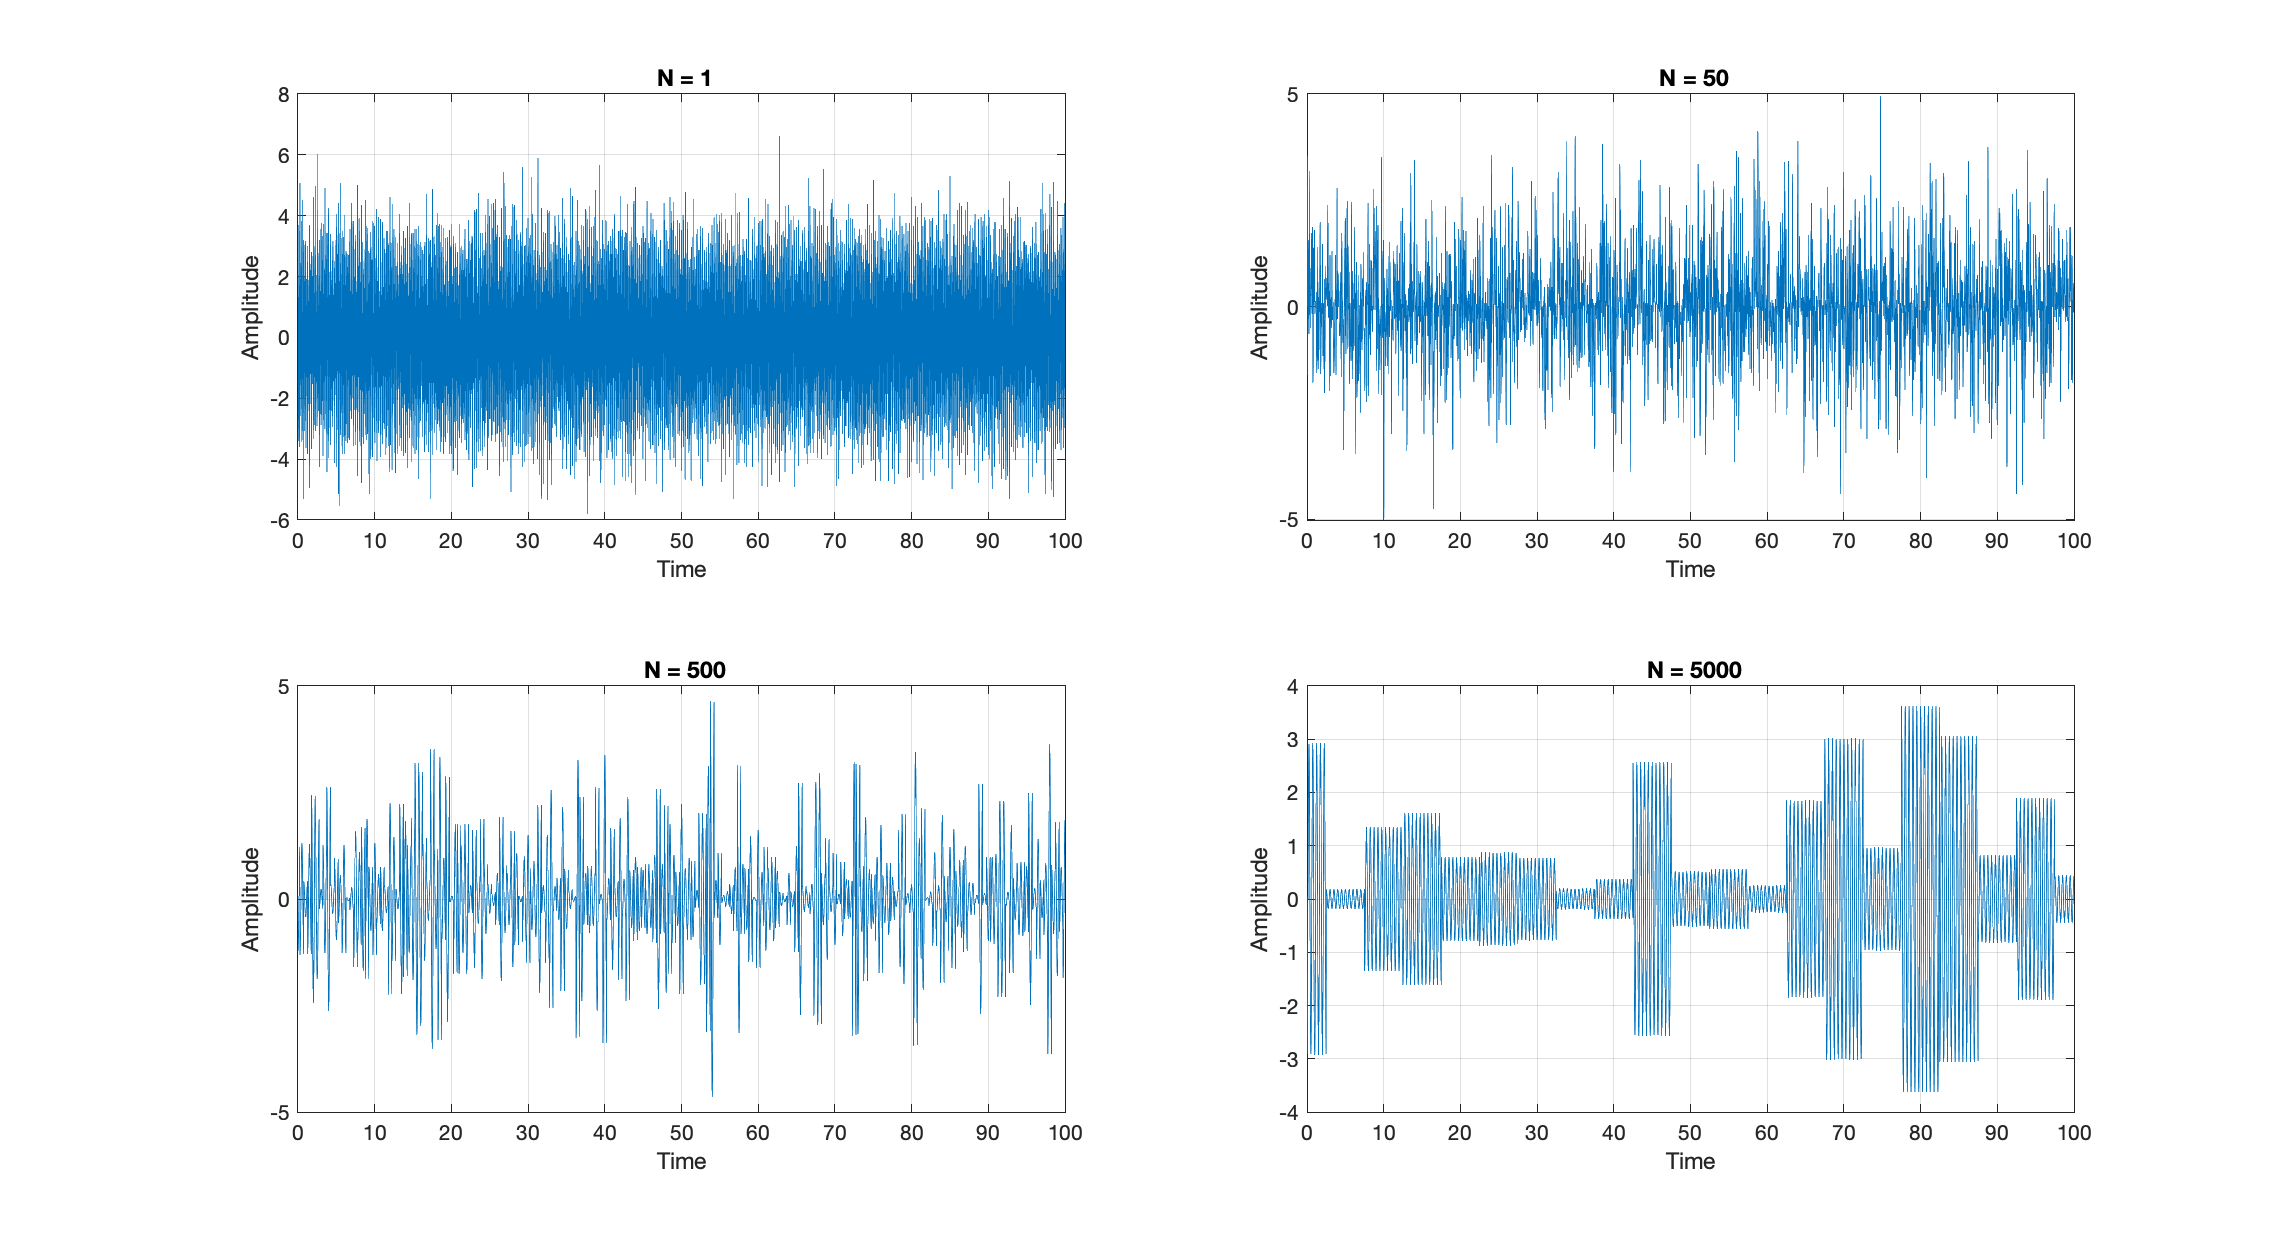
\includegraphics[width=1\linewidth]{../pics/q1-4}
 	\caption{خروجی کانال برای هر یک از  
 	\lr{N}
 های مشخص شده}
 	\label{fig:q1-4}
 \end{figure}

\noindent
همان‌طور که ملاحضه می‌شود، با کاهش N خروجی کانال تصادفی تر می‌شود چرا که عملا نمونه های بیشتری از کانال‌های تصادفی با پارامترهای متفاوت‌تری عبور کرده‌اند و به همین دلیل خروجی برای N های کمتر، تصادفی‌تر می‌شود.
 \newpage
 \section{بازیابی سیگنال خروجی از کانال چند مسیره}
 \subsection{محاسبه پارامترهای جبران‌ساز}
 هدف ما این است که پاسخ فرکانسی کل سیستم متشکل از کانال و جبران‌ساز با هم، از معادله
  \eqref{eq1}
  پیروی کند.
  \begin{equation}\label{eq1}
  	H_{Eq}(f) H_{C}(f) = ke^{-j2\pi ft_0}
  \end{equation}
در نتیجه داریم:
\begin{equation}
	\begin{split}
		H_{Eq}(f) &= \frac{ke^{-j2\pi ft_0}}{\sum_{i=1}^{n} a_i e^{-j2\pi f \tau_i}} \\
		&= \frac{1}{\sum_{i=1}^{n} \frac{a_i e^{-j2\pi f \tau_i}}{ke^{-j2\pi ft_0}}} \\
		&= \frac{1}{\sum_{i=1}^{n} \frac{a_i}{k} e^{-j2\pi f(\tau_i - t_0)}}
	\end{split}
\end{equation}
حال برای آنکه تابع به شکل خواسته شده در بیاید باید مقادیر
$t_0$
و 
$k$
را به شکل زیر قرار دهیم
\begin{equation}
	\begin{cases}
		&k = a_1\\
		&t_0 = \tau_1 
	\end{cases}
\end{equation}

با قرار دادن این مقادیر به شکل بالا، برای تابع نهایی داریم:
\begin{equation}
	H_{Eq}(f) = \frac{1}{1 + \sum_{i=2}^{n} \frac{a_i}{a_1} e^{-j2\pi f(\tau_i - \tau_1)}}
\end{equation}
پس برای مقادیر 
$k_i$
و
$t_i$
خواسته شده داریم:
 \begin{equation}
 	\begin{cases}
 		&k_i = \frac{a_i}{a_1} \\
 		&t_i = \tau_i - \tau_1 
 	\end{cases}
 \end{equation}
\newpage
\subsection{ساختار جبران‌ساز}
طبق بسط تیلور داریم:
\[\frac{1}{1+x} = 1 - x + x^2 - x^3 + x^4 - \dots\]
پس برای 
$H_{Eq}(f)$
نیز داریم:
\begin{equation}\label{eq6}
\begin{split}
	H_{Eq}(f) &= \frac{1}{1 + \sum_{i=2}^{n} k_i e^{-j2\pi f t_i} } \\
	&= 1 - \sum_{i=2}^{n} k_i e^{-j2\pi f t_i} + (\sum_{i=2}^{n} k_i e^{-j2\pi f t_i})^2 - \dots
\end{split}
\end{equation}
حال اگر جملات با توان های بالاتر را نیز باز کنیم، پاسخ نهایی به شکل جمع یکسری 
$b_i e^{-j2\pi f\tau_i^\prime}$
در می‌آید. حال اگر این جملات را به ترتیب 
$\tau_i^\prime$
ها از کوچک تر به بزرگ تر مرتب کنیم، در نهایت تابع به شکل معادله زیر در می‌آید.
\begin{equation}\label{eq7}
	H_{Eq}(f) = 1 + \sum_{i = 1}^{\infty} C_i e^{-j2\pi f \tau_i^\prime}
\end{equation}
جملات به دست آمده در معادله
 \eqref{eq7}
 در حوزه زمان، پاسخ ضربه‌ای مطابق با معادله 
 \eqref{eq8}
را شکل می‌دهند.
\begin{equation}\label{eq8}
	h_{Eq}(t) = \delta(t) + \sum_{i=1}^{\infty}C_i \delta(t-\tau_i^\prime)
\end{equation}
حال اگر 
$T_i$
را به شکل 
$T_i = \tau_i^\prime - \tau_{i-1}^\prime$
تعریف کنیم، خواهیم داشت:
\begin{equation}\label{eq9}
	h_{Eq}(t) = \delta(t) + \sum_{i=1}^{\infty} C_i \delta(t - \sum_{j=1}^{i} T_i)
\end{equation}
اگر در این پاسخ ضربه، فقط 
$m+1$
جمله اول را نگه داریم، خواهیم داشت:
\begin{equation}
	h_{Eq}(t) = \delta(t) + \sum_{i=1}^{m} C_i \delta(t - \sum_{j=1}^{i} T_i)
\end{equation}
که این پاسخه ضربه، در حقیقت نمایش دهنده پاسخ ضربه همان سیستم نمایش داده شده می‌باشد که در آن 
$C_0 = 1$
می‌باشد.

\newpage
\subsection{نمودار سیگنال ورودی}
نمودار مورد نظر در شکل 
\ref{fig:q2-3}
رسم شده است.
\begin{figure}[h]
	\centering
	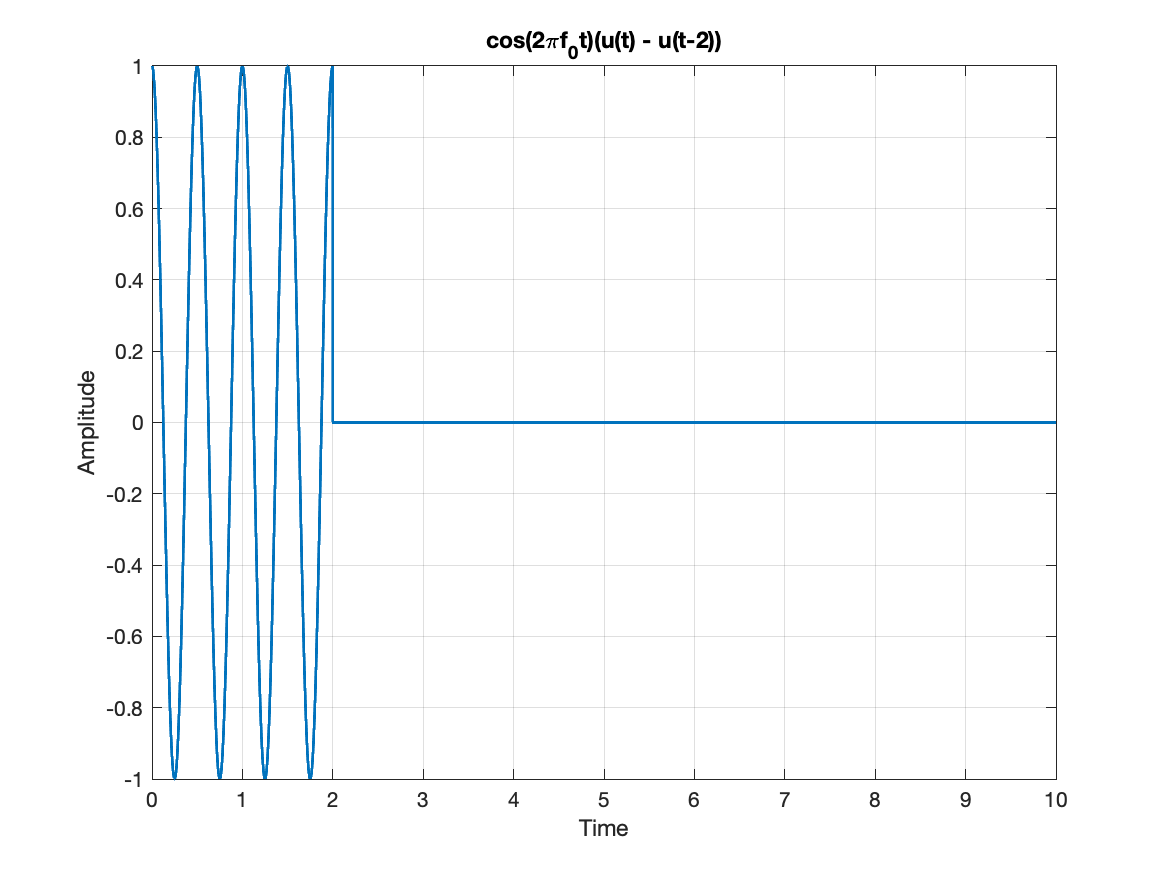
\includegraphics[width=1\linewidth]{../pics/q2-3}
	\caption{نمودار سیگنال ورودی بر حسب زمان}
	\label{fig:q2-3}
\end{figure}
\newpage
\subsection{پاسخ فرکانسی کانال}
برای کانال داده شده، رابطه پاسخ فرکانسی برابر است با:
\begin{equation}
	H(f) = e^{-j2\pi 5f} + 0.4e^{-j2\pi 5.01f}
\end{equation}
همچنین نمودار اندازه و فاز پاسخ فرکانسی این کانال مطابق شکل 
\ref{fig:q2-4}
می‌باشد.
\begin{figure}[h!]
	\centering
	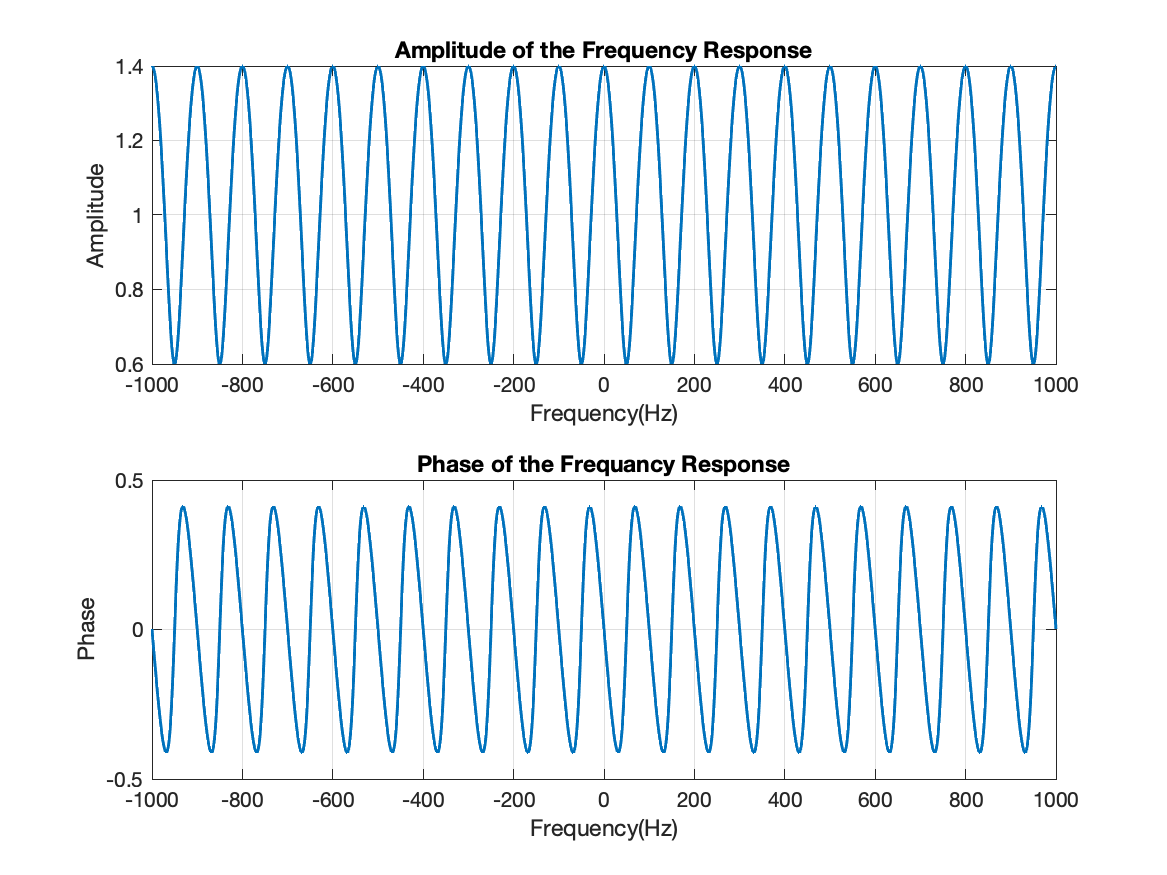
\includegraphics[width=0.9\linewidth]{../pics/q2-4}
	\caption{نمودار اندازه و فاز پاسخ فرکانسی کانال}
	\label{fig:q2-4}
\end{figure}
\newpage
\subsection{مقایسه ورودی و خروجی کانال}
در شکل زیر، نمودار ورودی و خروجی کانال به صورت همزمان رسم شده است.
\begin{figure}[h]
	\centering
	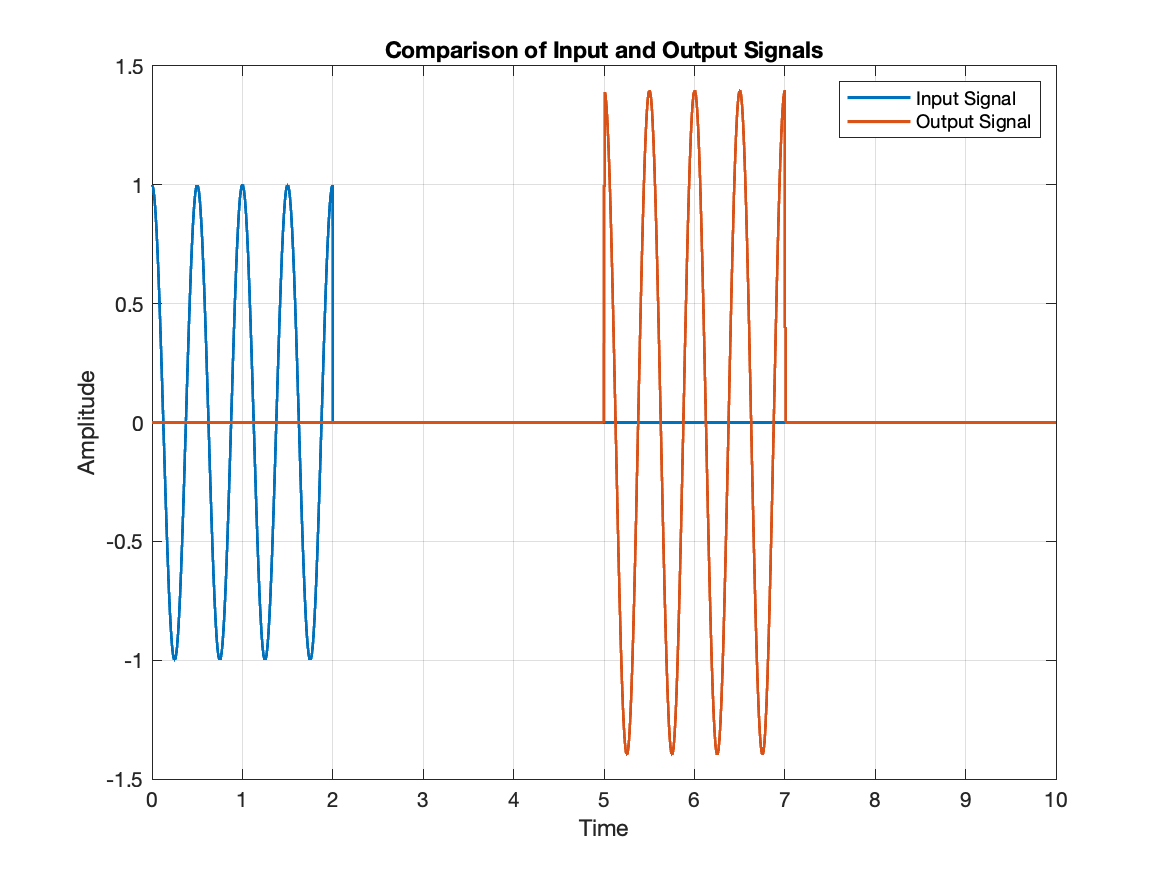
\includegraphics[width=0.9\linewidth]{../pics/q2-5}
	\caption{نمودار ورودی و خروجی کانال}
	\label{fig:q2-5}
\end{figure}

\noindent
برای تولید خروجی از دو متغیر 
\lr{$y_1$}
و 
\lr{$y_2$}
در کد متلب استفاده شده است که هرکدام برابرند با:
\begin{equation*}
	\begin{cases}
		& y_1(t) = x(t-5)\\
		& y_2(t) = 0.5x(t-5.01)
	\end{cases}
\end{equation*}
و در نهایت 
\lr{$y = y_1 + y_2$}
قرار داده شده است.
\newpage
\subsection{بازیابی سیگنال}
برای بازیابی سیگنال، با استفاده از معادله
 \eqref{eq6}
داریم:
\begin{equation}
	\begin{split}
		H_{Eq}(f) &= \frac{1}{1 + 0.4e^{-j2\pi 0.01f}}\\
		&= 1 + \sum_{i=1}^{\infty} (-0.4e^{-j2\pi 0.01f})^i
	\end{split}
\end{equation}
در نتیجه معادله بالا، برای میزان تاخیر و 
\lr{$C_i$}
ها داریم:
\begin{equation}
	\begin{cases}
		&C_i = (-0.4)^i \\
		&T_i = 0.01
	\end{cases}
\end{equation}

\noindent
حال برای محاسبه خطا خواسته شده، ابتدا تابعی به نام 
\lr{channel\_equalizer}
تعریف می‌کنیم که ورودی آن 
m
می‌باشد و خروجی آن سیگنال بازسازی شده می‌باشد. همچنین نمودار میزان خطا بر حسب m به شکل زیر می‌باشد.
\begin{figure}[h]
	\begin{center}
		\subfigure[اسکیل خطی]{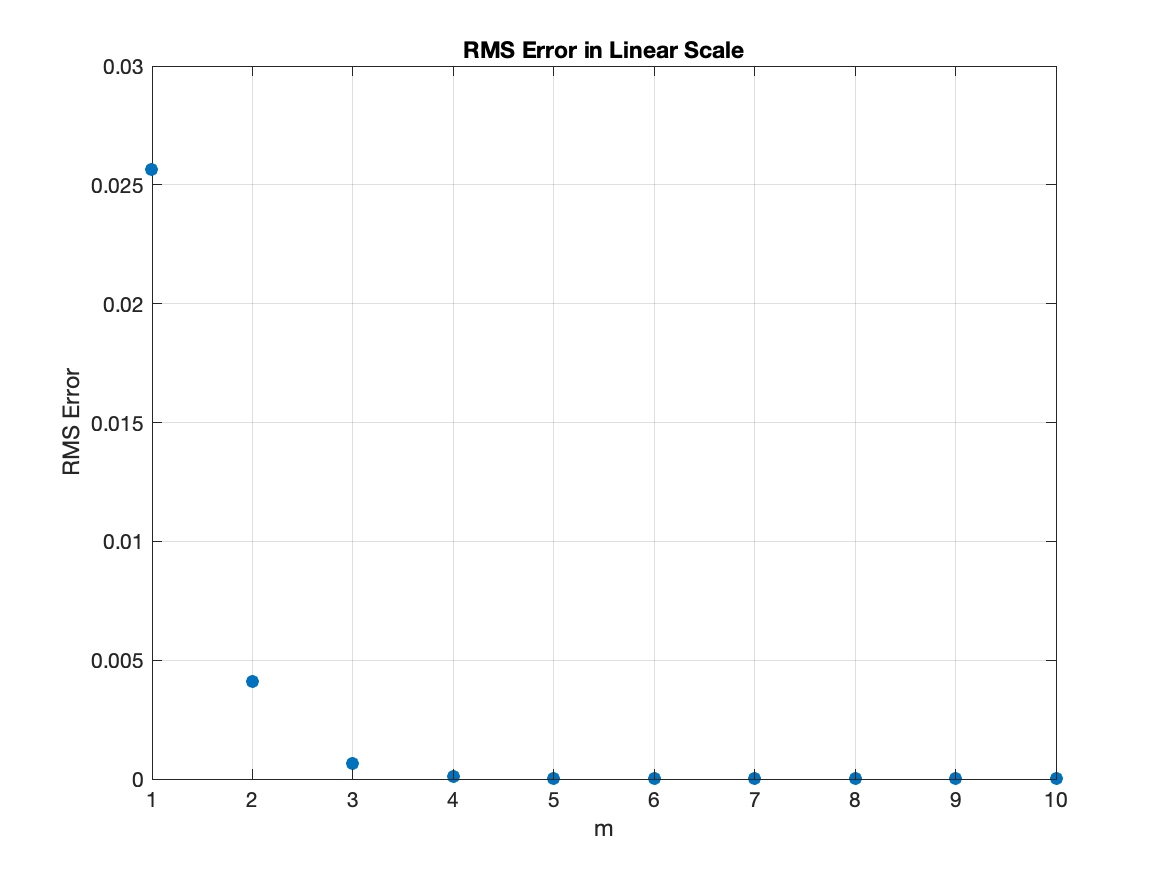
\includegraphics[width=2.8in]{../pics/q2-6-1}}
		\hspace{1cm}	
		\subfigure[اسکیل لگاریتمی]{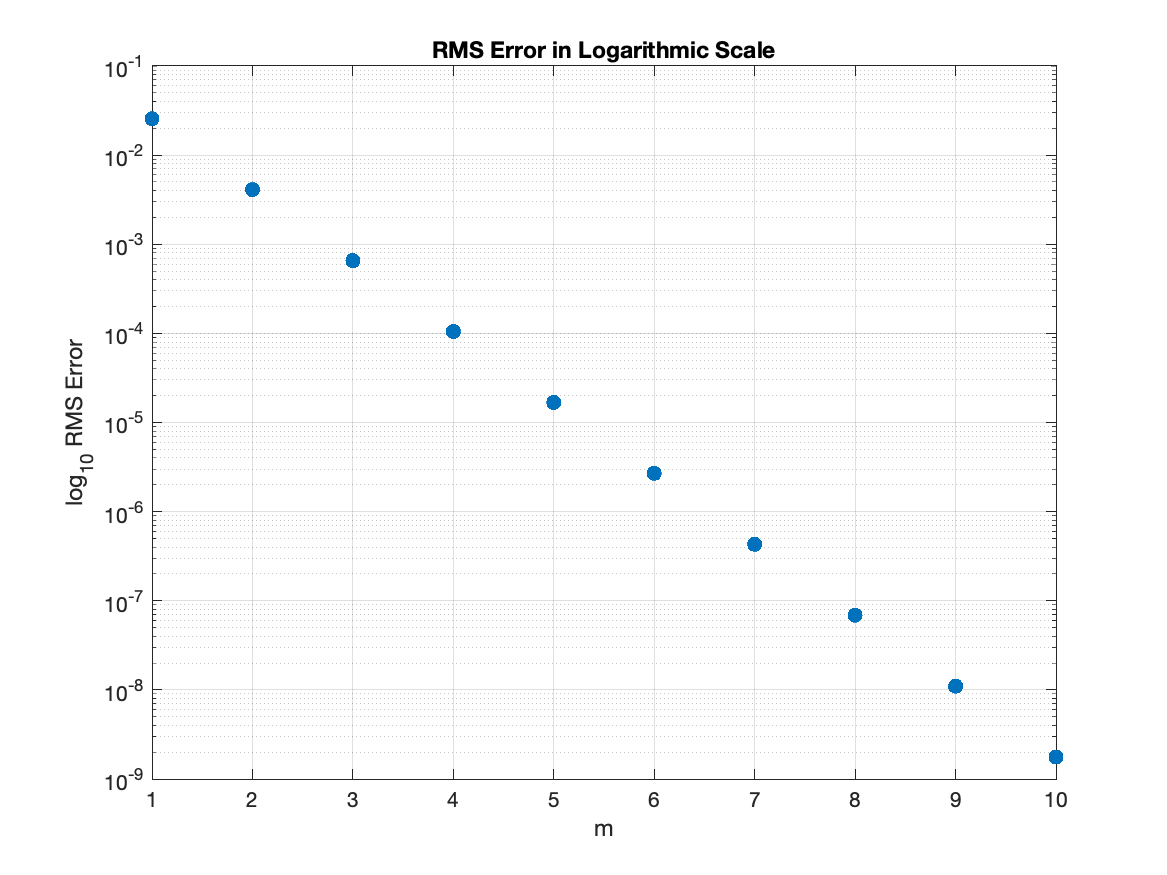
\includegraphics[width=2.8in]{../pics/q2-6-2}}
	\end{center}
	\caption{نمودار میزان خطا بر حسب m}
\end{figure}
\newpage
\subsection{مقایسه سیگنال‌ها}
با رسم هر چهار سیگنال خواسته شده، خروجی مطابق شکل زیر می‌شود.
\begin{figure}[h]
	\centering
	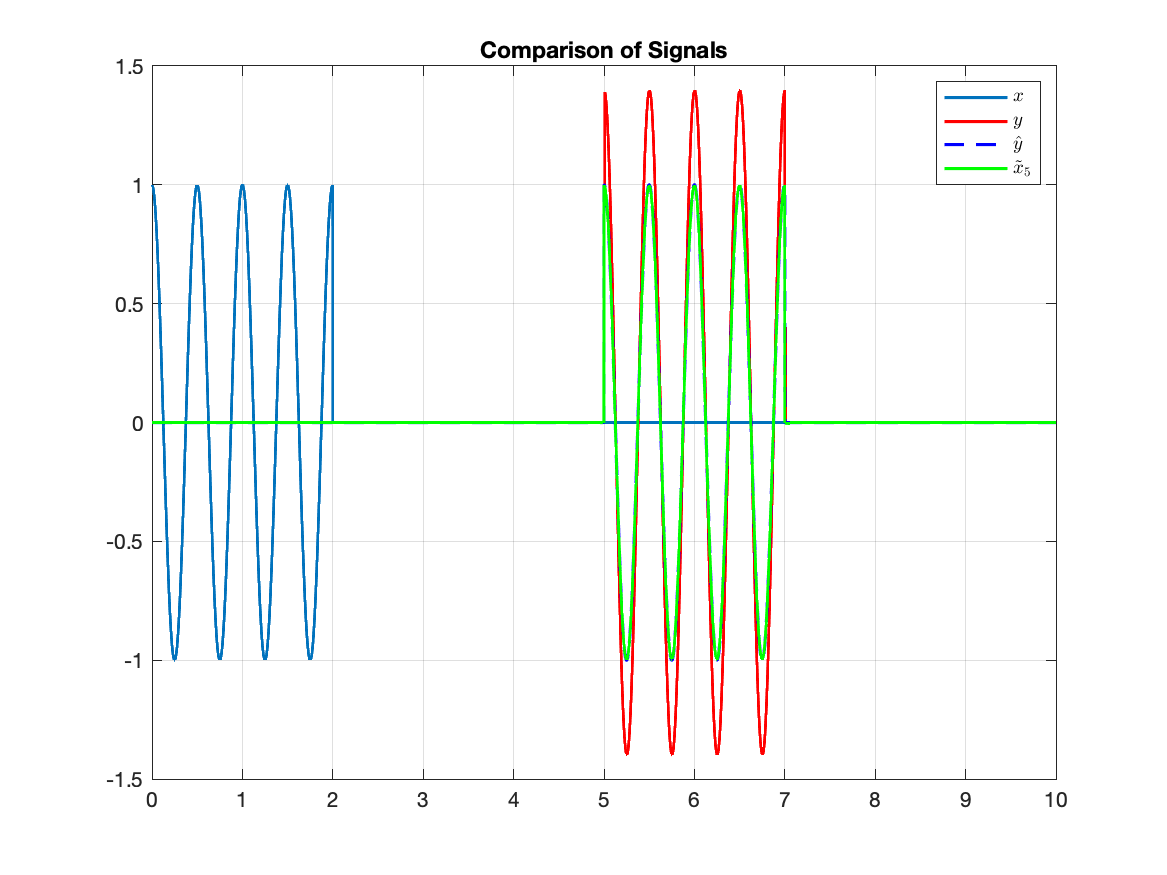
\includegraphics[width=1.1\linewidth]{../pics/q2-7}
	\caption{نمودار سیگنال‌های ورودی، خروجی، ایده آل و بازسازی شده}
	\label{fig:q2-7}
\end{figure}
همان‌طور که مشاهده می‌شود، سیگنال 
$\hat{y}$
که همان خروجی از کانال ایده‌آل می‌باشد،‌ تنها به مقدار ۵ ثانیه نسبت به سیگنال ورودی شیفت داده شده است. همان‌طور که دیده می‌شود، سیگنال 
$\tilde{x}_5$
به خوبی سیگنال 
$\hat{y}$
را بازسازی کرده است و این درحالی است که خروجی کانال غیر ایده‌آل یعنی 
$y$
دارای تفاوت‌های محسوسی نسبت به خروجی ایده آل می‌باشد. 


\end{document}